\ylDisplay{Kaheksa} % Ülesande nimi
{EFO žürii} % Autor
{piirkonnavoor} % Voor
{2018} % Aasta
{P 2} % Ülesande nr.
{1} % Raskustase
{
% Teema: Mehaanika

\ifStatement
 Kaheksakujulisel ringrajal alustavad kaks drooni võidusõitu ringide ühenduskohast nooltega $A$ ja $B$ näidatud suundades. Mõlema drooni trajektoorid on kaheksakujulised. Kaheksa ülemise osa pikkus on $l_A = 60$ $m$ ning alumise osa pikkus $l_B = 200$ $m$. Mõlemad droonid lendavad kogu aeg ühtlase kiirusega. Esimese drooni kiirus on $v_A = 10$ $m/s$ ning teise drooni kiirus $v_B = 8$ $m/s$. Kui suure teepikkuse $s$ on läbinud droon $A$, kui droonid uuesti kohtuvad? 
\begin{center}
	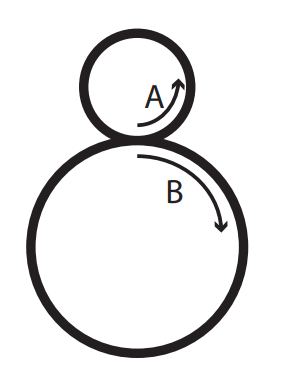
\includegraphics[width=0.5\linewidth]{2018-v2p-02-yl.PNG}
\end{center}
\fi

\ifHint
Ülesande lahendamisel tuleb hinnata kui palju on droon $A$ teisest droonist taga pool ning millise suhtelise kiirusega ta seda vahemaad läbib.
\fi

\ifSolution
Droon $A$ on droonist $B$ $s_A = 60$ $m$ tagapool. Drooni $A$ suhteline kiirus drooni $B$ suhtes
\begin{center}
$v = 10 m/s - 8 m/s = 2$ m/s.
\end{center}
Seega kulub droonil $A$ droonile $B$ järele jõudmiseks
\begin{center}
$t = v_A t = 10 m/s \cdot 30 s = 300$ m.
\end{center}
\fi
}
